
\begin{figure*}[htp]
	\centering
	\resizebox{\textwidth}{!}{%
		\begin{tikzpicture}[>=Stealth,
	entityStyle/.style={draw, color=white, thin, align=center, circle, text width=20mm},
	us/.style = {entityStyle, fill=amber},
	entity/.style={entityStyle, fill=azure},
	arrowStyle/.style={-latex', >=stealth },
	entityId/.style={draw, color=white,  thin, align=center, circle},]
	
	\node[us] (us) {\textbf{U.S}};
	
	\begin{scope}[every node/.style={entity}]
		\node[above left=2cm of us, xshift=-20mm] (c1) {\textbf{Donald Trump}};
		\node[above right=2cm of us, xshift=1cm] (c2) {\textbf{Jeff Bezos}};
		\node[below left=2cm of us, xshift=-20mm] (c3) {\textbf{New York}};
		\node[below right=2cm of us, xshift=1cm] (c4) {\textbf{Tesla Inc.}};
		
		\node[below left=3cm of c1, yshift=25mm, xshift=-15mm] (c1x) {\textbf{Melania Trump}};
		\node[above left=3cm of c3, yshift=-25mm, xshift=-15mm] (c3x) {\textbf{Tom Cruise}};
		
		%\node[left=1cm of c1x, yshift=25mm, xshift=-15mm] (c8) {\textbf{Thanh}};
	\end{scope}
	
	%\draw[->, line width=0.8mm, azure] (c8) -> (c1x);
	%\path[arrowStyle] (c8)--node[rotate=-31, yshift=4mm]{friend\_of} %node[rotate=-31, yshift=-3mm]{} (c1x);
	
	\foreach \value in {1,...,4}
	\draw[->, line width=0.8mm, azure] (c\value) -> (us);
	\foreach \value in {1,3}
	\draw[->, line width=0.8mm, azure] (c\value x) -> (c\value);
	
	\foreach \value in {1,3}
	\draw[->, line width=0.8mm, azure!60, dash pattern=on 3mm off 1mm, postaction={decorate}] (c\value x) -> (us);
	
	\path[arrowStyle] (c1)--node[rotate=-31, yshift=4mm]{president\_of} node[rotate=-31, yshift=-3mm]{$\alpha_{i4}$} (us);
	
	\path[arrowStyle] (c3)--node[rotate=30, yshift=4mm]{state\_of} node[rotate=30, yshift=-4mm]{$\alpha_{i3}$} (us);
	
	\path[arrowStyle] (c2)--node[rotate=41, yshift=4mm]{richest\_of} node[rotate=41, yshift=-4mm]{$\alpha_{i1}$} (us);
	
	\path[arrowStyle] (c4)--node[rotate=-41, yshift=4mm]{founded\_in} node[rotate=-41, yshift=-4mm]{$\alpha_{i2}$} (us);
	
	\path[arrowStyle] (c1x)--node[rotate=15, yshift=4mm]{wife\_of} (c1);
	\path[arrowStyle] (c3x)--node[rotate=-15, yshift=4mm]{born\_in} (c3);
	
	\path[arrowStyle] (c1x)--node[rotate=-8, yshift=4mm]{\textbf{first\_lady}} node[rotate=-8, yshift=-3mm]{$\alpha_{i5}$} (us);
	\path[arrowStyle] (c3x)--node[rotate=8, yshift=4mm]{\textbf{native\_of}} node[rotate=8, yshift=-3mm]{$\alpha_{i6}$} (us);
	
	%%%%%%%%%%%
	\node[entityId][fill=amber][right=11cm of us] (country) {$e_3$};
	\path[arrowStyle] (us)--node[yshift=2mm]{\LARGE $\rightarrow$} (country);
	
	\begin{scope}[every node/.style={entityId, fill=azure}]
		\node[above left=1cm of country, xshift=-5mm] (c1s) {$e_2$};
		\node[above right=1cm of country, xshift=5mm] (c2s) {$e_4$};
		\node[below left=1cm of country, xshift=-5mm] (c3s) {$e_6$};
		\node[below right=1cm of country, xshift=5mm] (c4s) {$e_7$};
		
		\node[below left=1.5cm of c1s, yshift=15mm, xshift=-5mm] (c1xs) {$e_1$};
		\node[above left=1.5cm of c3s, yshift=-15mm, xshift=-5mm] (c3xs) {$e_5$};
	\end{scope}
	\foreach \value in {1,...,4}
	\draw[->, line width=0.8mm, azure] (c\value s) -> (country);
	\foreach \value in {1,3}
	\draw[->, line width=0.8mm, azure] (c\value xs) -> (c\value s);
	
	\foreach \value in {1,3}
	\draw[->, line width=0.8mm, azure!60, dash pattern=on 3mm off 1mm, postaction={decorate}] (c\value xs) -> (country);
	
	\path[arrowStyle] (c1s)--node[rotate=-31, yshift=2mm]{$r_2$} (country);
	
	\path[arrowStyle] (c3s)--node[rotate=30, yshift=2mm]{$r_5$} (country);
	
	\path[arrowStyle] (c2s)--node[rotate=41, yshift=2mm]{$r_3$} (country);
	
	\path[arrowStyle] (c4s)--node[rotate=-41, yshift=2mm]{$r_6$} (country);
	
	\path[arrowStyle] (c1xs)--node[rotate=15, yshift=2mm]{$r_1$} (c1s);
	\path[arrowStyle] (c3xs)--node[rotate=-15, yshift=2mm]{$r_4$} (c3s);
	
	\path[arrowStyle] (c1xs)--node[rotate=-8, yshift=2mm]{$r_7$} (country);
	\path[arrowStyle] (c3xs)--node[rotate=8, yshift=2mm]{$r_8$} (country);
\end{tikzpicture}
	}
	\caption{Knowledge graph and normalized attention coefficients of the entity}
	\label{fig:graphExample}
\end{figure*}


\section{Related Work}
\label{chap:RelatedWork}

In this section, we present the basic definitions of knowledge graphs in order to understand the task of link prediction in knowledge graphs, as well as other related research directions.

\subsection{Definition of Knowledge Graphs}

The basic definitions of knowledge graphs are compiled and categorized by Cai, Hongyun \cite{cai2018comprehensive} and Goyal, Palash \cite{goyal2018graph} as follows:

%\begin{figure}[htp]
%	\centering
%	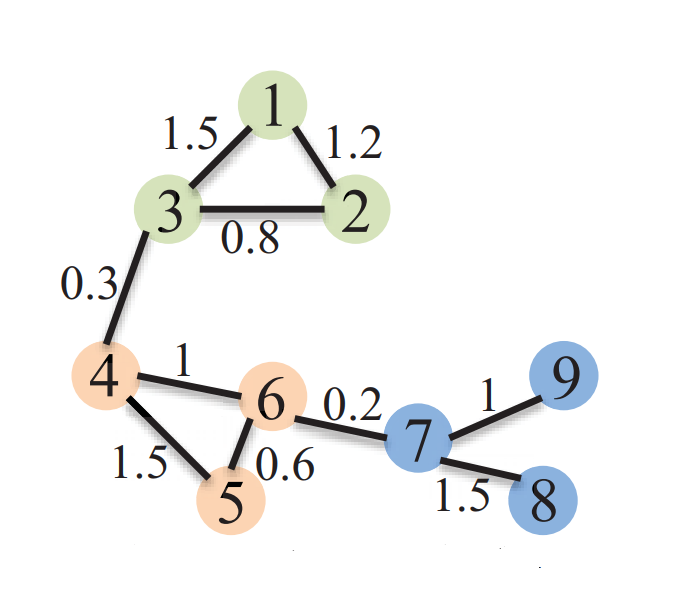
\includegraphics[width=7 cm]{figures/graph_emb_1.png}
%	\caption{Example of an input graph}
%	\label{fig:graphInput}
%\end{figure}


\begin{itemize}
	\item \begin{definition}[Graph]\label{def:defGraph}
		\(\mathcal{G} = (V, E)\), where \(v \in V\) is a vertex and \(e \in E\) is an edge. \(\mathcal{G}\) is associated with a vertex-type mapping function \(f_v: V \to T^v\) and an edge-type mapping function \(f_e: E \to T^e\).
	\end{definition}
	
	Here, \(T^v\) and \(T^e\) are the sets of vertex types and edge types, respectively. Each vertex \(v_i \in V\) belongs to a specific type, i.e., \(f_v(v_i) \in T^v\). Similarly, for \(e_{ij} \in E, f_e (e_{ij}) \in T^e\).
	
	\item
	\begin{definition}[Homogeneous Graph]\label{def:homogeneous}
		Homogeneous graph: \textit{ $\mathcal{G}_{homo} = (V, E)$ is a graph where $\mid T^v \mid = \mid T^e \mid = 1$. All vertices in $\mathcal{G}$ belong to a single type, and all edges belong to a single type}.
	\end{definition}
	
	\item
	\begin{definition}[Heterogeneous Graph]\label{def:heterogeneous}
		Heterogeneous graph: \textit{$\mathcal{G}_{hete} = (V, E)$ is a graph where $\mid T^v \mid > 1$ or $\mid T^e \mid > 1$. That is, there is more than one type of vertex or more than one type of edge}.
	\end{definition}
	
	\item
	\begin{definition}[Knowledge Graph]\label{def:knowledgeGraph}
		Knowledge graph:
		$\mathcal{G}_{know} = (V, R, E)$ is a directed graph, where the vertex set represents entities, the relation set represents relationships between entities, and the edge set $E \subseteq V\times R \times V$ represents events in the form of subject-property-object triples. Each edge is a triple $(\text{entity}_{\text{head}}, \text{relation}, \text{entity}_{\text{tail}})$ (denoted as $\langle h, r, t \rangle$), expressing a relation $r$ from head entity $h$ to tail entity $t$.
	\end{definition}
	
	Here, $h, t \in V$ are entities and $r \in R$ is a relation. We refer to $\langle h, r, t \rangle$ as a knowledge graph triple.
	
	Example: in \autoref{fig:graphExample}, there are two triples: 
	$\langle \text{Tom Cruise, born\_in, New York} \rangle$
	and $\langle \text{New York, state\_of, U.S} \rangle$. Note that entities and relations in a knowledge graph often belong to different types. Therefore, a knowledge graph can be viewed as a specific case of a heterogeneous graph.
\end{itemize}

\subsection{Link Prediction in Knowledge Graphs}


Link prediction, also known as knowledge graph completion, is the task of exploiting known facts (events) in a knowledge graph to infer missing ones. This is equivalent to predicting the correct tail entity in a triple $\langle h, r, ? \rangle$ (tail prediction) or the correct head entity in $\langle ?, r, t \rangle$ (head prediction). For simplicity, instead of distinguishing between head and tail prediction, we generally refer to the known entity as the \textit{source entity} and the entity to be predicted as the \textit{target entity}.

Most current research on link prediction in knowledge graphs is related to approaches that focus on embedding a given graph into a low-dimensional vector space. In contrast to these approaches is a rule-based method explored in \cite{burl}. Its core algorithm samples arbitrary rules and generalizes them into Horn clauses \cite{wiki:Horn}, then uses statistics to compute the confidence of these generalized rules. When predicting a new link (edge) in the graph, the task is to infer whether an edge with a specific label exists between two given nodes. Many methods have been proposed to learn rules from graphs, such as in RuDiK \cite{ortona2018robust}, AMIE \cite{galarraga2015fast}, and RuleN \cite{meilicke2018fine}.

As mentioned earlier, there are two main approaches to this problem: one is optimizing an objective function to find a small set of rules that cover the majority of correct examples with minimal error, as explored in RuDiK \cite{ortona2018robust}. The other approach, which we adopt in this thesis, aims to explore all possible rules and then generate a top-\(k\) ranking of candidate triples, each associated with a confidence score measured on the training set.

% GAT
In the deep learning branch of approaches, many successful techniques from image processing and natural language processing have been applied to knowledge graphs, such as Convolutional Neural Networks (CNNs \cite{lecun1999object}), Recurrent Neural Networks (RNNs \cite{hopfield2007hopfield}), and more recently, Transformers \cite{yang2019xlnet} and Capsule Neural Networks (CapsNets \cite{sabour2017dynamic}). In addition, other techniques such as random walks and hierarchical structure-based models have also been explored. The common advantage of these deep learning methods on knowledge graphs is their ability to automatically extract features and generalize complex graph structures based on large amounts of training data. However, some methods focus mainly on grid-like structures and fail to preserve the spatial characteristics of knowledge graphs.

The attention mechanism, particularly the multi-head attention layer, has been applied to graphs through the Graph Attention Network (GAT \cite{velivckovic2017graph}) model, which aggregates information about an entity based on attention weights from its neighboring entities. However, GAT lacks integration of relation embeddings and the embeddings of an entity's neighbors—components that are crucial for capturing the role of each entity. This limitation has been addressed in the work \textit{Learning Attention-based Embeddings for Relation Prediction in Knowledge Graphs} (\textbf{KBAT} \cite{nathani2019learning}), which we adopt as the foundation for our study.


The attention mechanism is currently one of the most effective (state-of-the-art) deep learning structures, as it has been proven to substitute any convolution operation \cite{cordonnier2019relationship}. Moreover, it serves as a core component in leading models for natural language processing, such as Megatron-LM \cite{shoeybi2019megatron}, and image segmentation, such as HRNet-OCR (Hierarchical Multi-Scale Attention \cite{tao2020hierarchical}). Some recent works \cite{cordonnier2020multi} have proposed interesting improvements based on the attention mechanism. However, these advancements have not yet been applied to knowledge graphs, which motivates us to adopt this family of methods to integrate the latest innovations into knowledge graph modeling.


\begin{figure*}[htbp]
	\centering
	\tikzset{
		category/.style  = {draw, thin, align=center},
		subcat/.style={rectangle, rounded corners=6pt},
		center/.style = {category, ellipse, fill=blue!60, text width=4em},
		group/.style = {category, subcat, fill=blue!30, rounded corners=3pt, text width=6em},
		yellowbox/.style = {category, subcat, fill=yellow!30},
		greenbox/.style = {category, subcat, fill=green!30},
		redbox/.style = {category, subcat, fill=red!30},
		bluebox/.style = {category, subcat, fill=cyan!30},
		leafbox/.style = {category, subcat, fill=black!10, rounded corners=3pt}
	}
	\resizebox{1\textwidth}{!}{%
		\begin{tikzpicture}
	\node[center][execute at begin node=\setlength{\baselineskip}{0.9em}] (root) {Knowledge Graph};
	\node[group][above left=1cm of root, execute at begin node=\setlength{\baselineskip}{1em}] (c1) {Knowledge Representation Learning};
	\node[group][above right=8mm of root, execute at begin node=\setlength{\baselineskip}{1em}] (c2) {Knowledge Inference};
	\node[group][below left=5mm of root, execute at begin node=\setlength{\baselineskip}{1em}] (c3) {Knowledge Acquisition};
	\node[group][below right=20mm of root, xshift=-2cm, execute at begin node=\setlength{\baselineskip}{0.9em}] (c4) {Temporal Knowledge Graph};
	
	\begin{scope}[every node/.style={yellowbox}]
		\node[above=8mm of c1, xshift=-1cm] (c11) {Embedding Space};
		\node[left=of c1, yshift=9mm, xshift=-7mm, yshift=10mm] (c12) {Scoring Function};
		\node[left=15mm of c1, yshift=-5mm] (c13) {Model Encoding};
		\node[left=of c1, yshift=-20mm] (c14) {Auxiliary Information};
	\end{scope}
	
	\begin{scope}[every node/.style={redbox}]
		\node[above left=of c2, text width=35mm, yshift=1mm, xshift=14mm, execute at begin node=\setlength{\baselineskip}{0.9em}] (c21) {Natural Language Understanding};
		\node[above=1cm of c2, yshift=5mm, xshift=13mm] (c22) {Question Answering};
		\node[right=of c2, yshift=15mm] (c23) {Dialogue System};
		\node[right=of c2, yshift=4mm, xshift=7mm] (c24) {Recommendation System};
		\node[below=5mm of c2, xshift=5mm] (c25) {Other Applications};
	\end{scope}
	
	\begin{scope}[every node/.style={greenbox}]
		\node[left=1cm of c3, yshift=5mm] (c31) {Entity Discovery};
		\node[below left=of c3, yshift=8mm, xshift=3mm] (c32) {Relation Extraction};
		\node[below right=10mm of c3, xshift=-4cm] (c33) {Graph Completion};
	\end{scope}
	
	\begin{scope}[every node/.style={bluebox}]
		\node[below=of c4, xshift=-15mm, yshift=-37mm] (c41) {Temporal Logic Reasoning};
		\node[below=of c4, xshift=18mm, yshift=-25mm] (c42) {Time-Independent Relations};
		\node[below right=of c4, xshift=0mm, yshift=-15mm] (c43) {Dynamic Entities};
		\node[right=of c4, xshift=11mm, yshift=-22mm] (c44) {Temporal Embeddings};
	\end{scope}
	
	\begin{scope}[every node/.style={leafbox}]
		\node[above=5mm of c11] (c11x) {
			\begin{tabular}{@{}l@{}@{}l@{}}
				- Point-wise & - Manifold \\
				- Complex & - Gaussian \\
				- Discrete & \\
			\end{tabular}
		};
		\node[above=5mm of c12, xshift=-5mm] (c12x) {
			\begin{tabular}{@{}l@{}}
				- Distance-based \\
				- Semantic \\
				- Others \\
			\end{tabular}
		};
		\node[left=of c13, yshift=5mm] (c13x) {
			\begin{tabular}{@{}l@{}}
				- Linear / Bilinear \\
				- Matrix Factorization \\
				- Neural Nets \\
				- CNN \\
				- RNN \\
				- Transformers \\
				- GCN \\
			\end{tabular}
		};
		\node[below left=5mm of c14, xshift=6mm, yshift=-3mm] (c14x) {
			\begin{tabular}{@{}l@{}c@{}l@{}}
				- Textual & - Type & - Visual \\
			\end{tabular}
		};
		%%%%%%%%%%%% 
		\node[below left=of c31] (c31x) {
			\begin{tabular}{@{}l@{}}
				- Recognition \\
				- Typing \\
				- Disambiguation \\
				- Ranking \\
			\end{tabular}
		};
		\node[below=of c32, xshift=-7mm] (c32x) {
			\begin{tabular}{@{}l@{}}
				- Neural Nets \\
				- Attention \\
				- GCN \\
				- GAN \\
				- RL \\
				- Others \\
			\end{tabular}
		};
		\node[below=5mm of c33, xshift=2mm] (c33x) {
			\begin{tabular}{@{}l@{}}
				- Ranking-based Embeddings \\
				- Textual Reasoning \\
				- Rule-based Reasoning \\
				- Hyper-relational Learning \\
				- Triple Classification \\
			\end{tabular}
		};
		%%%%%%%%%%%%%%%%%
		\node[above=5mm of c22] (c22x) {
			\begin{tabular}{@{}l@{}}
				- Single-fact QA \\
				- Multi-step Reasoning \\
			\end{tabular}
		};
		\node[below right=5mm of c25, yshift=18mm] (c25x) {
			\begin{tabular}{@{}l@{}}
				- Question Generation \\
				- Search Engines \\
				- Medical Applications \\
				- Health Recovery \\
				- Zero-shot Image Classification \\
				- Text Generation \\
				- Semantic Analysis \\
			\end{tabular}
		};
	\end{scope}
	
	\foreach \value in {1,...,4}
	\draw[->, very thick] (root) -> (c\value);
	
	\foreach \value in {1,...,4}
	\draw[->, thick] (c1) -> (c1\value);
	\foreach \value in {1,...,4}
	\draw[->, thick] (c1\value) -> (c1\value x);
	
	\foreach \value in {1,...,5}
	\draw[->, thick] (c2) -> (c2\value);
	\foreach \value in {2,5}
	\draw[->, thick] (c2\value) -> (c2\value x);
	
	\foreach \value in {1,...,3}
	\draw[->, thick] (c3) -> (c3\value);
	\foreach \value in {1,...,3}
	\draw[->, thick] (c3\value) -> (c3\value x);
	
	\foreach \value in {1,...,4}
	\draw[->, thick] (c4) -> (c4\value);
	
\end{tikzpicture}
	}
	\caption{
		A taxonomy of research areas in knowledge graphs}
	\label{fig:categoriesResearch}
\end{figure*}


\subsection{Research Areas in Knowledge Graphs}


Knowledge representation has a long-standing history in logic and artificial intelligence. In the context of knowledge graphs, four major research areas have been categorized and summarized in the survey \cite{ji2020survey}, including: Knowledge Representation Learning, Knowledge Acquisition, Temporal Knowledge Graphs, and Knowledge-aware Applications. All research categories are illustrated in \autoref{fig:categoriesResearch}.

\textbf{Knowledge Representation Learning}

Knowledge representation learning is an essential research topic in knowledge graphs that enables a wide range of real-world applications. It is categorized into four subgroups:

\begin{itemize}
	\item \textit{Representation Space} focuses on how entities and relations are represented in vector space. This includes point-wise, manifold, complex vector space, Gaussian distribution, and discrete space embeddings.
	
	\item \textit{Scoring Function} studies how to measure the validity of a triple in practice. These scoring functions may be distance-based or similarity-based.
	
	\item \textit{Encoding Models} investigate how to represent and learn interactions among relations. This is currently the main research direction, including linear or non-linear models, matrix factorization, or neural network-based approaches.
	
	\item \textit{Auxiliary Information} explores how to incorporate additional information into embedding models, such as textual, visual, and type information.
\end{itemize}

\textbf{Knowledge Acquisition}

Knowledge acquisition focuses on how to extract or obtain knowledge based on knowledge graphs, including knowledge graph completion, relation extraction, and entity discovery. Relation extraction and entity discovery aim to extract new knowledge (relations or entities) into the graph from text. Knowledge graph completion refers to expanding an existing graph by inferring missing links. Research directions include embedding-based ranking, relation path reasoning, rule-based reasoning, and hyper-relational learning.

Entity discovery tasks include entity recognition, disambiguation, typing, and ranking. Relation extraction models often employ attention mechanisms, graph convolutional networks (GCNs), adversarial training, reinforcement learning (RL), deep learning, and transfer learning, which is the foundation of the method proposed in our work.

In addition, other major research directions in knowledge graphs include \textbf{temporal knowledge graphs} and \textbf{knowledge-aware applications}. Temporal knowledge graphs incorporate temporal information into the graph to learn temporal representations. Knowledge-aware applications include natural language understanding, question answering, recommendation systems, and many other real-world tasks where integrating knowledge improves representation learning.



% All text must be in a two-column format.
% The total allowable size of the text area is $6\frac78$ inches (17.46 cm) wide by $8\frac78$ inches (22.54 cm) high.
% Columns are to be $3\frac14$ inches (8.25 cm) wide, with a $\frac{5}{16}$ inch (0.8 cm) space between them.
% The main title (on the first page) should begin 1 inch (2.54 cm) from the top edge of the page.
% The second and following pages should begin 1 inch (2.54 cm) from the top edge.
% On all pages, the bottom margin should be $1\frac{1}{8}$ inches (2.86 cm) from the bottom edge of the page for $8.5 \times 11$-inch paper;
% for A4 paper, approximately $1\frac{5}{8}$ inches (4.13 cm) from the bottom edge of the
% page.

% %-------------------------------------------------------------------------
% \subsubsection{Margins and page numbering}

% All printed material, including text, illustrations, and charts, must be kept
% within a print area $6\frac{7}{8}$ inches (17.46 cm) wide by $8\frac{7}{8}$ inches (22.54 cm)
% high.
% %
% Page numbers should be in the footer, centered and $\frac{3}{4}$ inches from the bottom of the page.
% The review version should have page numbers, yet the final version submitted as camera ready should not show any page numbers.
% The \LaTeX\ template takes care of this when used properly.



% %-------------------------------------------------------------------------
% \subsubsection{Type style and fonts}

% Wherever Times is specified, Times Roman may also be used.
% If neither is available on your word processor, please use the font closest in
% appearance to Times to which you have access.

% MAIN TITLE.
% Center the title $1\frac{3}{8}$ inches (3.49 cm) from the top edge of the first page.
% The title should be in Times 14-point, boldface type.
% Capitalize the first letter of nouns, pronouns, verbs, adjectives, and adverbs;
% do not capitalize articles, coordinate conjunctions, or prepositions (unless the title begins with such a word).
% Leave two blank lines after the title.

% AUTHOR NAME(s) and AFFILIATION(s) are to be centered beneath the title
% and printed in Times 12-point, non-boldface type.
% This information is to be followed by two blank lines.

% The ABSTRACT and MAIN TEXT are to be in a two-column format.

% MAIN TEXT.
% Type main text in 10-point Times, single-spaced.
% Do NOT use double-spacing.
% All paragraphs should be indented 1 pica (approx.~$\frac{1}{6}$ inch or 0.422 cm).
% Make sure your text is fully justified---that is, flush left and flush right.
% Please do not place any additional blank lines between paragraphs.

% Figure and table captions should be 9-point Roman type as in \cref{fig:onecol,fig:short}.
% Short captions should be centred.

% \noindent Callouts should be 9-point Helvetica, non-boldface type.
% Initially capitalize only the first word of section titles and first-, second-, and third-order headings.

% FIRST-ORDER HEADINGS.
% (For example, {\large \bf 1. Introduction}) should be Times 12-point boldface, initially capitalized, flush left, with one blank line before, and one blank line after.

% SECOND-ORDER HEADINGS.
% (For example, { \bf 1.1. Database elements}) should be Times 11-point boldface, initially capitalized, flush left, with one blank line before, and one after.
% If you require a third-order heading (we discourage it), use 10-point Times, boldface, initially capitalized, flush left, preceded by one blank line, followed by a period and your text on the same line.

% %-------------------------------------------------------------------------
% \subsubsection{Footnotes}

% Please use footnotes\footnote{This is what a footnote looks like.
% It often distracts the reader from the main flow of the argument.} sparingly.
% Indeed, try to avoid footnotes altogether and include necessary peripheral observations in the text (within parentheses, if you prefer, as in this sentence).
% If you wish to use a footnote, place it at the bottom of the column on the page on which it is referenced.
% Use Times 8-point type, single-spaced.


% %-------------------------------------------------------------------------
% \subsubsection{Cross-references}

% For the benefit of author(s) and readers, please use the
% {\small\begin{verbatim}
%   \cref{...}
% \end{verbatim}}  command for cross-referencing to figures, tables, equations, or sections.
% This will automatically insert the appropriate label alongside the cross-reference as in this example:
% \begin{quotation}
%   To see how our method outperforms previous work, please see \cref{fig:onecol} and \cref{tab:example}.
%   It is also possible to refer to multiple targets as once, \eg~to \cref{fig:onecol,fig:short-a}.
%   You may also return to \cref{sec:formatting} or look at \cref{eq:also-important}.
% \end{quotation}
% If you do not wish to abbreviate the label, for example at the beginning of the sentence, you can use the
% {\small\begin{verbatim}
%   \Cref{...}
% \end{verbatim}}
% command. Here is an example:
% \begin{quotation}
%   \Cref{fig:onecol} is also quite important.
% \end{quotation}

% %-------------------------------------------------------------------------
% \subsubsection{References}

% List and number all bibliographical references in 9-point Times, single-spaced, at the end of your paper.
% When referenced in the text, enclose the citation number in square brackets, for
% example~\cite{Authors14}.
% Where appropriate, include page numbers and the name(s) of editors of referenced books.
% When you cite multiple papers at once, please make sure that you cite them in numerical order like this \cite{Alpher02,Alpher03,Alpher05,Authors14b,Authors14}.
% If you use the template as advised, this will be taken care of automatically.

% \begin{table}
%   \centering
%   \caption{\label{tab:example}%
%     Results.
%     Ours is better.
%   }
%   \begin{tabular}{lc}
%     \toprule
%     Method & Frobnability \\
%     \midrule
%     Theirs & Frumpy \\
%     Yours & Frobbly \\
%     Ours & Makes one's heart Frob\\
%     \bottomrule
%   \end{tabular}
% \end{table}

% %-------------------------------------------------------------------------
% \subsubsection{Illustrations, graphs, and photographs}

% All graphics should be centered.
% In \LaTeX, avoid using the \texttt{center} environment for this purpose, as this adds potentially unwanted whitespace.
% Instead use
% {\small\begin{verbatim}
%   \centering
% \end{verbatim}}
% at the beginning of your figure.
% Please ensure that any point you wish to make is resolvable in a printed copy of the paper.
% Resize fonts in figures to match the font in the body text, and choose line widths that render effectively in print.
% Readers (and reviewers), even of an electronic copy, may choose to print your paper in order to read it.
% You cannot insist that they do otherwise, and therefore must not assume that they can zoom in to see tiny details on a graphic.

% When placing figures in \LaTeX, it's almost always best to use \verb+\includegraphics+, and to specify the figure width as a multiple of the line width as in the example below
% {\small\begin{verbatim}
%    \usepackage{graphicx} ...
%    \includegraphics[width=0.8\linewidth]
%                    {myfile.pdf}
% \end{verbatim}
% }


% %-------------------------------------------------------------------------
% \subsubsection{Color}

% Please refer to the author guidelines on the \confName\ \confYear\ web page for a discussion of the use of color in your document.

% If you use color in your plots, please keep in mind that a significant subset of reviewers and readers may have a color vision deficiency; red-green blindness is the most frequent kind.
% Hence avoid relying only on color as the discriminative feature in plots (such as red \vs green lines), but add a second discriminative feature to ease disambiguation.